% A test file for the module "diagtikz.lua" of dednat6.
% This file: http://angg.twu.net/dednat6/demo-tikz.tex.html
%            http://angg.twu.net/dednat6/demo-tikz.tex
%                         (find-dednat6 "demo-tikz.tex")
%    Output: http://angg.twu.net/dednat6/demo-tikz.pdf
%
% (defun c () (interactive) (find-dednat6sh "lualatex -record demo-tikz.tex"))
% (defun d () (interactive) (find-pdf-page "~/dednat6/demo-tikz.pdf"))
% (defun e () (interactive) (find-dednat6 "demo-tikz.tex"))
% (defun u () (interactive) (find-latex-upload-links "demo-tikz"))
%   (find-pdf-page "~/dednat6/demo-tikz.pdf")
% http://angg.twu.net/dednat6/demo-tikz.pdf
%
\documentclass[oneside]{article}
\usepackage[colorlinks,citecolor=DarkRed,urlcolor=DarkRed]{hyperref} % (find-es "tex" "hyperref")
\usepackage[x11names,svgnames]{xcolor} % (find-es "tex" "xcolor")
%
%\usepackage{proof}  % For derivation trees ("%:" lines)
\input diagxy        % For 2D diagrams ("%D" lines)
\xyoption{curve}     % For the ".curve=" feature in 2D diagrams
%
\usepackage{tikz}
%
\begin{document}
  \catcode`\^^J=10                      % (find-es "luatex" "spurious-omega")
  \directlua{dofile "dednat6load.lua"}  % (find-dednat6 "dednat6load.lua")

\def\defdiagtikz#1#2{\expandafter\def\csname diagtikz-#1\endcsname{#2}}
\def\ifdiagtikzundefined#1{\expandafter\ifx\csname diagtikz-#1\endcsname\relax}
\def\diagtikz#1{\ifdiagtikzundefined{#1}
    \errmessage{UNDEFINED DIAGTIKZ: #1}
  \else
    \csname diagtikz-#1\endcsname
  \fi
}

% A poor man's "\verb"
\def\co#1{{%
  \def\\{\char92}%
  \def\%{\char37}%
  \tt#1%
  }}
\def\qco#1{`\co{#1}'}








\title{Dednat6: a demo for diagtikz.lua}
\author{Eduardo Ochs}
\date{}
\maketitle

Dednat6 can generate Tikz code for diagrams instead of diagxy code,
but the current support for Tikz is a currently a very minimal
prototype that only supports a few kinds of arrows --- namely
\qco{->}, \qco{|->}, and \qco{=>} ---, it ignores the modifers for
labels, placement, slides, and curve, and it generates Tikz code that
looks awful when rendered... the two diagrams below were generated
from \qco{\%D}-blocks that were almost identical, but the first one
used \qco{diagram test-diagxy} and \qco{enddiagram} and the second one
used \qco{tikzdiagram test-tikz} and \qco{endtikzdiagram}.

%L require "diagtikz"
%
%D diagram test-diagxy
%D 2Dx     100   +40
%D 2D  100 A --> B
%D 2D            |
%D 2D  +30       C
%D 2D
%D (( A B ->  .plabel= a foo
%D    B C =>  .plabel= r bar
%D    A C |-> .plabel= m plic
%D ))
%D enddiagram
%D
%D tikzdiagram test-tikz
%D 2Dx     100   +40
%D 2D  100 A --> B
%D 2D            |
%D 2D  +30       C
%D 2D
%D (( A B ->  .plabel= a foo
%D    B C =>  .plabel= r bar
%D    A C |-> .plabel= m plic
%D ))
%D endtikzdiagram

\pu

%% The code above generates this:
%
% \defdiag{test-diagxy}{
%   \morphism(0,0)|a|/->/<600,0>[{A}`{B};{foo}]
%   \morphism(600,0)|r|/=>/<0,-450>[{B}`{C};{bar}]
%   \morphism(0,0)|m|/|->/<600,-450>[{A}`{C};{plic}]
% }
% \defdiagtikz{test-tikz}{
%   \begin{tikzpicture}
%     \node (100 100) at (0.0,0.0) {$A$};
%     \node (140 100) at (2.0,0.0) {$B$};
%     \node (140 130) at (2.0,-1.5) {$C$};
%     \draw [->]            (100 100) -- (140 100);
%     \draw [{}-{>},double] (140 100) -- (140 130);
%     \draw [{|}-{>}]       (100 100) -- (140 130);
%   \end{tikzpicture}}

$$\diag{test-diagxy}
  \quad
  \diagtikz{test-tikz}
$$

\bigskip

The Tikz code generated for the second diagrams is:

\begin{verbatim}
  \defdiagtikz{test-tikz}{
    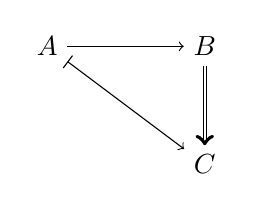
\begin{tikzpicture}
      \node (100 100) at (0.0,0.0) {$A$};
      \node (140 100) at (2.0,0.0) {$B$};
      \node (140 130) at (2.0,-1.5) {$C$};
      \draw [->]            (100 100) -- (140 100);
      \draw [{}-{>},double] (140 100) -- (140 130);
      \draw [{|}-{>}]       (100 100) -- (140 130);
    \end{tikzpicture}}
\end{verbatim}

The problem is that I know very little Tikz! If you know how to make
the Tikz code above better --- how to fix the double arrow, how to add
the labels, whatever --- please get in touch!

\bigskip

The source of this file is here:

% \medskip

\url{http://angg.twu.net/dednat6/demo-tikz.tex.html}

\url{http://angg.twu.net/dednat6/demo-tikz.tex}





\end{document}

% Local Variables:
% coding: utf-8-unix
% End:
